\documentclass{standalone}
\usepackage{tikz}
\usetikzlibrary{shapes.geometric, arrows}

\definecolor{mycolor}{RGB}{0, 153, 255}
\tikzstyle{process} = [rectangle, rounded corners,
                       minimum width=2cm, minimum height=1cm,
                       text centered, draw=black, fill=mycolor,
                       text=white, line width=0.3mm]

\tikzstyle{arrow} = [thick,->,>=stealth]

\begin{document}
    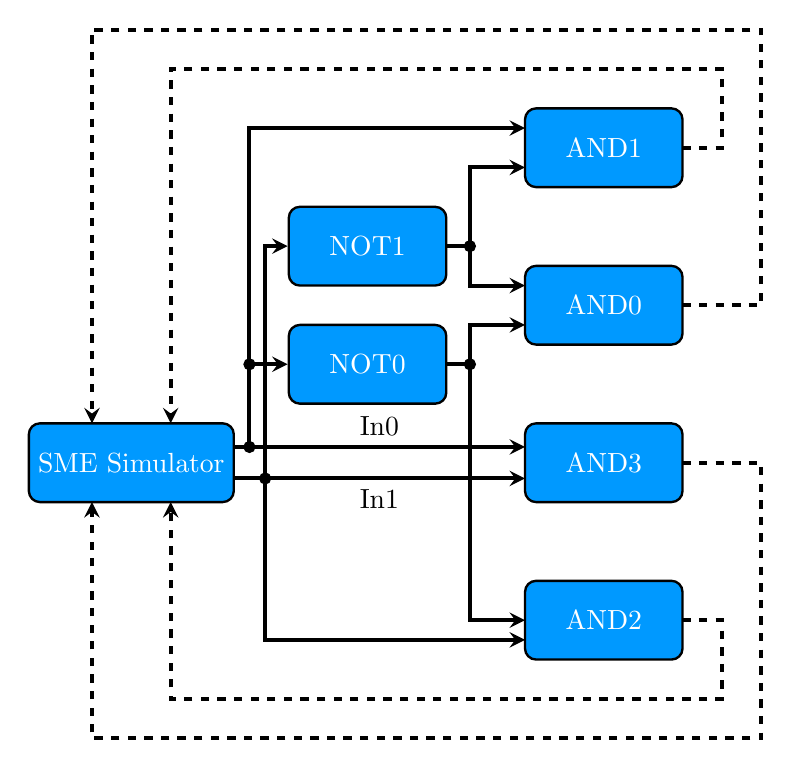
\begin{tikzpicture}[node distance=2cm]
        
        \node (Simulator) [process] {SME Simulator};
        
        %NOT Gates
        \node (NOT0) [process, right of = Simulator, xshift=1cm, yshift=1.25cm] {NOT0};
        \node (NOT1) [process, above of = NOT0, xshift=0cm, yshift=-0.5cm] {NOT1};
        
        %Simulator to NOT gates
        \draw [arrow, line width=0.5mm] (1.7, -0.2) |-  (NOT1);
        \filldraw[black] (1.7, -0.2) circle (2pt);
        \draw [arrow, line width=0.5mm] (1.5, 0.2) |-  (NOT0);
        \filldraw[black] (1.5, 0.2) circle (2pt);
        \filldraw[black] (1.5, 1.25) circle (2pt);
        
        %\draw [arrow, dashed, line width=0.5mm] (NOT0) -- ++(2, 0) |- (Simulator);
        
        %AND Gates
        \node (AND3) [process, right of = NOT0, xshift=1cm, yshift=-1.25cm] {AND3};
        \node (AND0) [process, above of = AND3, xshift=0cm] {AND0};
        \node (AND1) [process, above of = AND0, xshift=0cm] {AND1};
        \node (AND2) [process, below of = AND3, xshift=0cm] {AND2};
        
        %Lines to AND0 gates
        \draw [arrow, line width=0.5mm] (NOT1) -- ++(1.3,0) |-  (5, 2.25);
        \draw [arrow, line width=0.5mm] (NOT0) -- ++(1.3,0) |-  (5, 1.75);
        \filldraw[black] (4.3, 2.75) circle (2pt);
        
        %Lines to AND1 gates
        \draw [arrow, line width=0.5mm] (1.5,0.2) |-  (5, 4.25);
        \draw [arrow, line width=0.5mm] (NOT1) -- ++(1.3,0)  |-  (5,3.75);
        
        %Lines to AND2gates
        \draw [arrow, line width=0.5mm] (1.7,-0.2) |-  (5, -2.25);
        \draw [arrow, line width=0.5mm] (NOT0) -- ++(1.3,0)  |-  (5,-2);
        \filldraw[black] (4.3, 1.25) circle (2pt);

        %Lines to AND3 gates
        \draw [arrow, line width=0.5mm] (1.3,0.2) -- node [above] {In0} (5,0.2);
        \draw [arrow, line width=0.5mm] (1.3,-0.2) -- node [below] {In1} (5,-0.2);
        
        %Output lines to simulator
        %AND3
        \draw [arrow, line width=0.5mm, dashed] (7,0) -- ++(1, 0) -- ++(0,-3.5) -- ++(-8.5,0) -- (-0.5,-0.5);
        %AND2
        \draw [arrow, line width=0.5mm, dashed] (7,-2) -- ++(0.5, 0) -- ++(0,-1) -- ++(-7,0) -- (0.5,-0.5);
        %AND0
        \draw [arrow, line width=0.5mm, dashed] (7,2) -- ++(1, 0) -- ++(0,3.5) -- ++(-8.5,0) -- (-0.5,0.5);
        %AND1
        \draw [arrow, line width=0.5mm, dashed] (7,4) -- ++(0.5, 0) -- ++(0,1) -- ++(-7,0) -- (0.5,0.5);
        
    
    \end{tikzpicture}
\end{document}
